\documentclass[11pt,a4paper]{article}
\usepackage[utf8]{inputenc}
\usepackage[spanish]{babel}	%Idioma
\usepackage{amsmath}
\usepackage{amsfonts}
\usepackage{amssymb}
\usepackage{graphicx} 	%Añadir imágenes
\usepackage{geometry}	%Ajustar márgenes
\usepackage[export]{adjustbox}[2011/08/13]
\usepackage{float}
\restylefloat{table}
\usepackage[hidelinks]{hyperref}
\usepackage{titling}
\graphicspath{{/home/nazaret/Escritorio/LaTEX}}
\usepackage{subcaption} 
\usepackage{multirow}
\usepackage{caption}
\usepackage{multicol}
\usepackage[shortlabels]{enumitem}
\usepackage{array}
\selectlanguage{spanish}

%Opciones de encabezado y pie de página:
\usepackage{fancyhdr}
\pagestyle{fancy}
\lhead{Nazaret Román Guerrero}
\rhead{Procesamiento Digital de Señales}
\lfoot{Grado en Ingeniería Informática}
\cfoot{}
\rfoot{\thepage}
\renewcommand{\headrulewidth}{0.4pt}
\renewcommand{\footrulewidth}{0.4pt}

%Opciones de fuente:
\usepackage[utf8]{inputenc}
\usepackage[default]{sourcesanspro}
\usepackage{sourcecodepro}
\usepackage[T1]{fontenc}

\setlength{\parindent}{15pt}
\setlength{\headheight}{15pt}
\setlength{\voffset}{10mm}

% Custom colors
\usepackage{color}
\definecolor{deepblue}{rgb}{0,0,0.5}
\definecolor{deepred}{rgb}{0.6,0,0}
\definecolor{deepgreen}{rgb}{0,0.5,0}

\usepackage{listings}
\usepackage{color}
\usepackage{graphicx}

\definecolor{dkgreen}{rgb}{0,0.6,0}
\definecolor{gray}{rgb}{0.5,0.5,0.5}
\definecolor{mauve}{rgb}{0.58,0,0.82}

\lstset{frame=tb,
  language=Matlab,
  aboveskip=3mm,
  belowskip=3mm,
  showstringspaces=false,
  columns=flexible,
  basicstyle={\small\ttfamily},
  numbers=left,
  numberstyle=\tiny\color{gray},
  keywordstyle=\color{blue},
  commentstyle=\color{dkgreen},
  stringstyle=\color{mauve},
  breaklines=true,
  breakatwhitespace=true,
  tabsize=4
}

\begin{document}
\begin{titlepage}

\begin{minipage}{\textwidth}

\centering

\includegraphics[width=0.55\textwidth]{img/logo.png}\\

\textsc{\Large Procesamiento Digital de Señales\\[0.2cm]}
\textsc{GRADO EN INGENIERÍA INFORMÁTICA}\\[1cm]

{\Huge\bfseries Práctica 4\\}
\noindent\rule[-1ex]{\textwidth}{3pt}\\[3.5ex]
{\large\bfseries Sistemas Discretos. Transformada Z y respuesta en frecuencia}
\end{minipage}

\vspace{1.5cm}
\begin{minipage}{\textwidth}
\centering

\textbf{Autora}\\ {Nazaret Román Guerrero}\\[2.5ex]

\includegraphics[width=0.3\textwidth]{img/etsiit.jpeg}\\[0.1cm]
\vspace{1cm}
\textsc{Escuela Técnica Superior de Ingenierías Informática y de Telecomunicación}\\
\vspace{1cm}
\textsc{Curso 2018-2019}
\end{minipage}
\end{titlepage}

\pagenumbering{gobble}
\pagenumbering{arabic}
\tableofcontents
\thispagestyle{empty}

\newpage

Para esta práctica se ha utilizado un intérprete online de Matlab. Dicho intérprete es el mismo que en la anterior sesión y es el siguiente: \color{blue} \url{https://octave-online.net/}\color{black}.\\

Para sacar el plano Z vamos a usar la función \texttt{zplane()}.

\section{Transformada Z y función de transferencia}
\subsection{Filtro IIR y filtro IIR con la función \texttt{filter}}

	El código se puede ver en la sección \color{deepred}\nameref{code1}\color{black} y en \color{deepred}\nameref{code2}\color{black}. Ambos producen la misma salida. La única diferencia con respecto al código de la práctica anterior es que se calculan los polos del filtro, es decir, calculamos \texttt{roots(a)}.\\
	
	El código está incluido con el nombre de \texttt{iir\_impulso.m}. Al ejecutar el código, la salida es la siguiente:
	
	\begin{itemize}
		\item Primer polo: $(0 + 0.94868i)$
		\item Segundo polo: $(0 - 0.94868i)$
	\end{itemize}
	
\begin{figure}[H]
  \centering
  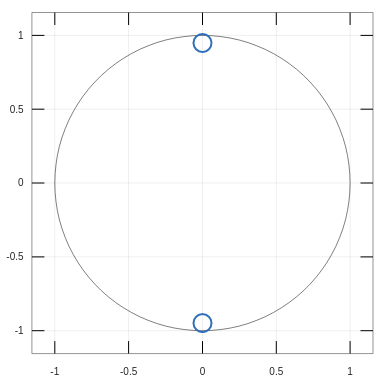
\includegraphics[width=0.5\linewidth]{img/polosg1.png}
\end{figure}
	
	Sabemos que un sistema es estable si se cumple que la región de convergencia (ROC a partir de ahora) de su función de transferencia se corresponde con el exterior de un círculo de radio $r<\infty$.\\
	
	También sabemos que un sistema causal es estable si la ROC de la funcion incluye la circunferencia unidad, es decir, los polos caen dentro del círculo de radio $r=1$.\\
	
	Teniendo esto en cuenta, podemos ver que el sistema es, en efecto, causal, ya que los polos caen dentro de un círculo con radio $r<\infty$, por ejemplo $r=0.08$.  También es estable puesto que los polos caen dentro la circunferencia de radio unidad.
	
\subsection{Filtro IIR con el escalón unitario}

El código está incluido con el nombre de \texttt{iir\_escalon.m} y también se puede ver en \color{deepred}\nameref{code3}\color{black}.\\

Puesto que la ecuación en diferencias es exactamente la misma que en el apartado anterior, el resultado de calcular los polos del denominador es el mismo. Por tanto, al ejecutar el código tenemos que:

	\begin{itemize}
		\item Primer polo: $(0 + 0.94868i)$
		\item Segundo polo: $(0 - 0.94868i)$
	\end{itemize}
	
\begin{figure}[H]
  \centering
  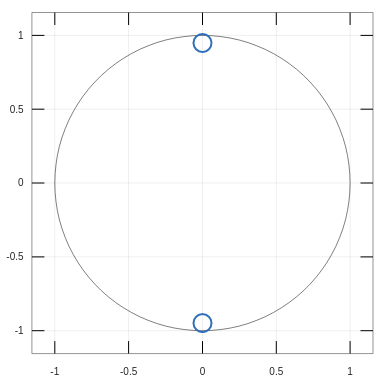
\includegraphics[width=0.5\linewidth]{img/polosg1.png}
\end{figure}

Por tanto

\begin{itemize}
	\item Causalidad: el sistema es causal para $r=0.8$.
	\item Estabilidad: el sistema es estable puesto que los polos están dentro de la circunferencia unidad.
\end{itemize}

\subsection{Filtro IIR con otra ecuación en diferencias}

Podemos encontrar el código en el \texttt{.zip} bajo el nombre de \texttt{iir\_otro.m} y en \color{deepred}\nameref{code4}\color{black}.\\

El resultado obtenido con este código es el siguiente:

\begin{itemize}
	\item Primer polo: $(2 + 0.0000i)$
   	\item Segundo polo: $(0.5 + 0.0000i)$
\end{itemize}

\begin{figure}[H]
  \centering
  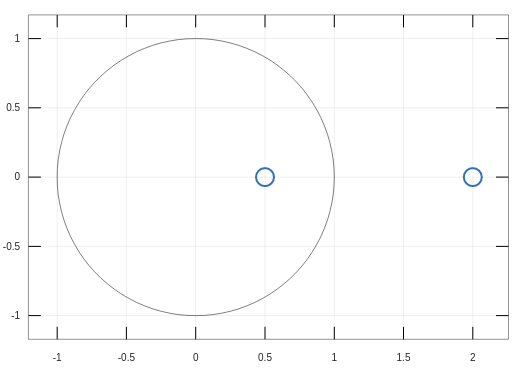
\includegraphics[width=0.7\linewidth]{img/polosg3.png}
\end{figure}

Observando los polos podemos decir:

\begin{itemize}
	\item Causalidad: el sistema es causal para $r=0.4$.
	\item Estabilidad: el sistema no es estable. Hay un polo que queda fuera de la circunferencia unidad.
\end{itemize}

\subsection{Filtro FIR con el impulso unitario}

El código se inlcuye con el nombre de \texttt{fir\_impulso.m}. Además, se puede ver el código en la sección \color{deepred}\nameref{code5}\color{black}.\\

Ejecutando el código obtenemos el siguiente resultado:

\begin{figure}[H]
  \centering
  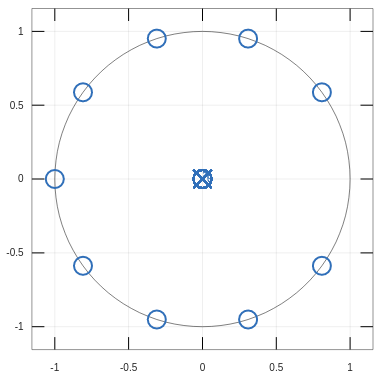
\includegraphics[width=0.5\linewidth]{img/polosg4.png}
\end{figure}

Los filtros FIR nunca tienen polos, solo ceros. Esto se debe a que los filtros FIR siempre son estables. Por tanto:

\begin{itemize}
	\item Causalidad: el sistema es causal para cualquier $r$.
	\item Estabilidad: el sistema es estable.
\end{itemize}

\subsection{Filtro FIR con el escalón unitario}

Este código se encuentra disponible en el \texttt{.zip} bajo el nombre de \texttt{fir\_escalon.m}. También está incluido en la sección \color{deepred}\nameref{code6}\color{black}.\\

Al ejecutarlo obtenemos la siguiente salida:

\begin{figure}[H]
  \centering
  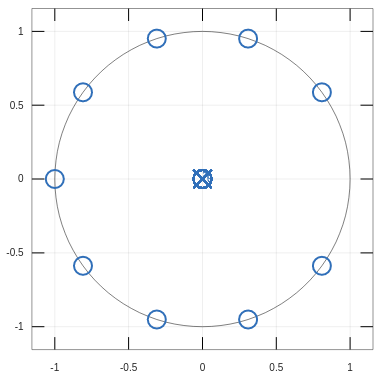
\includegraphics[width=0.45\linewidth]{img/polosg4.png}
\end{figure}

A la vista la imagen, podemos decir que:

\begin{itemize}
	\item Causalidad: el sistema es causal para cualquier $r$.
	\item Estabilidad: el sistema es un filtro FIR, por lo que no tiene polos, lo que significa que es estable.
\end{itemize}

\subsection{Filtro FIR con la función \texttt{conv}}

El código de este apartado está incluido como \texttt{fir\_conv.m} y en \color{deepred}\nameref{code7}\color{black}.\\

\begin{figure}[H]
  \centering
  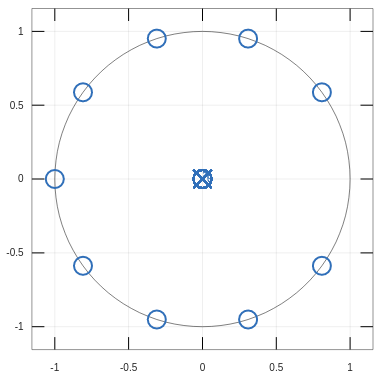
\includegraphics[width=0.5\linewidth]{img/polosg4.png}
\end{figure}

Al igual que en los dos filtros anteriores:

\begin{itemize}
	\item Causalidad: este sistema es causal para cualquier $r$.
	\item Estabilidad: el sistema es estable ya que es un filtro FIR.
\end{itemize}
\newpage

\section{Respuesta en frecuencia}

Ahora vamos a calcular la respuesta en frecuencia de los filtros IIR y FIR originales de la práctica anterior. Para ello vamos a utilizar la función \texttt{freqz}, que genera la respuesta del filtro que se le pase con la resolución que se le indique. A pesar de que se pide utilizar los cursores de Matlab, al utilizar un intérprete online estoy atada a las funciones que vengan implementadas. Por desgracia los cursores no están disponibles en el intérprete:

\begin{figure}[H]
	\centering
	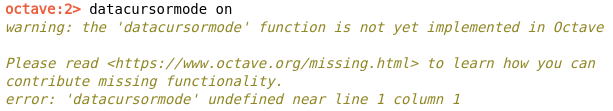
\includegraphics[scale=0.5]{img/cursor.png}
\end{figure}

\subsection{Filtro IIR}
El código de este ejercicio cambia, puesto que es un código nuevo y que calcula algo distinto a la práctica pasada. Por tanto, está incluido en el \texttt{.zip} bajo el nombre de \texttt{freqz\_iir.m}. Además, el código se puede ver también en la sección \color{deepred}\nameref{code8}\color{black}.\\

Como se puede ver, primero se establecen los coeficientes de la ecuación en diferencias del filtro y entonces se calcula la respuesta en frecuencia, estableciendo 1024 puntos para ello.

\begin{figure}[H]
	\centering
	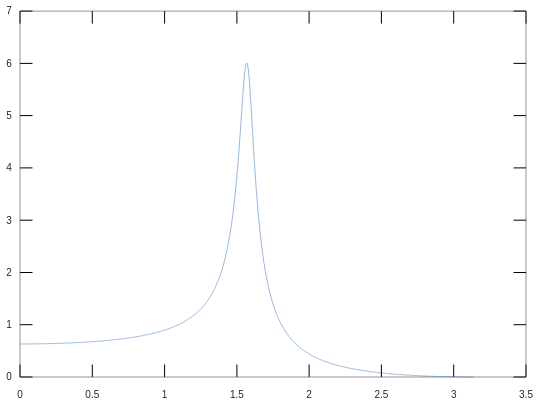
\includegraphics[scale=0.4]{img/freqz-iir.png}
\end{figure}

Como podemos ver gracias a la gráfica, el filtro es paso banda, ya que deja pasar algunas frecuencias concretas y rechaza las demás. Puesto que no puedo utilizar cursores, he intentado visualizar las frecuencias de corte aproximadas en la gráfica.\\

En este caso la frecuencia de corte es solo una, alrededor de 1.6 Hz. Puesto que no es un filtro ideal, deja pasar algunas frecuencias más, que varían entre 1.3 y 1.8 Hz aproximadamente.

\subsection{Filtro FIR}

Para este ejercicio, vamos a utilizar el filtro de la práctica anterior que tomaba 10 muestras y hacía la media para dar una salida. El código está incluido con el nombre de \texttt{freqz\_fir.m}, aunque el código también se puede leer en la sección \color{deepred}\nameref{code9}\color{black}.\\

Al igual que en el caso del filtro IIR, definimos los coeficientes de la ecuación en diferencias, teniendo en cuenta que se toman 10 muestras. Se calcula la respuesta en frecuencia y se genera la gráfica con los 1024 puntos que hemos indicado para calcularla. El resultado es el siguiente:

\begin{figure}[H]
	\centering
	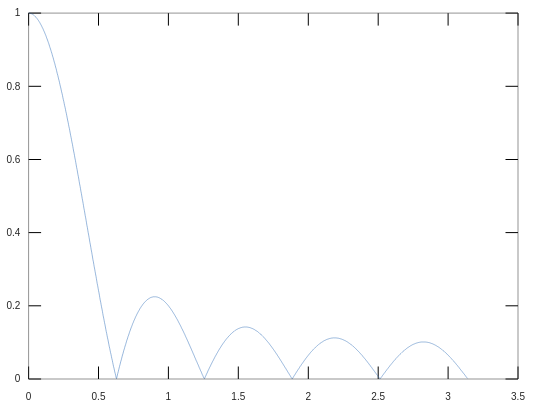
\includegraphics[scale=0.4]{img/freqz-fir.png}
\end{figure}

En este caso es un filtro paso baja, ya que deja pasar las frecuencias bajas y evita el paso de aquellas que son más grandes. Como no es un filtro perfecto, se generan pequeños picos pero a pesar de ello la tendencia del filtro es clara.\\

De nuevo he intentado determinar la frecuencia de corte mirando la gráfica, y aproximadamente diría que es 0.1 Hz, aunque en este caso es algo más complicado de vislumbrar porque la caída es brusca y casi al principio del eje X.

\newpage

\section{Anexo: Códigos fuente}

\subsection{Filtro IIR (impulso unitario)}
\label{code1}

\begin{lstlisting}[frame=single]
% Se define el array con los pulsos
x=[1 zeros(1,29)];

% Se definen los coeficientes de las ecuaciones en diferencias
a=[1 0 0.9];
b=[0.3 0.6 0.3];

% Muestra actual
xn=[0 0 0];
yn=[0 0 0];

for n=1:length(x)
	% Los valores cambian en cada vuelta
	xn(3)=xn(2); xn(2)=xn(1); xn(1)=x(n);

	yn(3)=yn(2); yn(2)=yn(1); yn(1)=0.;

	% Se calcula el resultado de operacion de filtrado
	y(n) = -a*yn' +b*xn';

	% Se actualizan los valores
	yn(1)=y(n);
end

% Pintamos la grafica discreta y continua
stem(y);

% Calculamos los polos
zplane(roots(a))
\end{lstlisting}

\subsection{Filtro IIR (impulso unitario) con \texttt{filter}}
\label{code2}

\begin{lstlisting}[frame=single]
% Se define el array con los pulsos
x=[1 zeros(1,29)];

% Se definen los coeficientes de las ecuaciones en diferencias
a=[1 0 0.9];
b=[0.3 0.6 0.3];

filtro = filter(b, a, x)

% Pintamos la grafica discreta y continua
stem(filtro);

% Calculamos los polos
zplane(roots(a))
\end{lstlisting}

\subsection{Filtro IIR (escalón unitario)}
\label{code3}

\begin{lstlisting}[frame=single]
% Se define el array con los pulsos
x=[ones(1,30)];

% Se definen los coeficientes de las ecuaciones en diferencias
a=[1 0 0.9];
b=[0.3 0.6 0.3];

filtro = filter(b, a, x)

% Pintamos la grafica discreta y continua
stem(filtro);

% Calculamos los polos del resultado
zplane(roots(a))
\end{lstlisting}

\subsection{Filtro IIR con otra ecuación en diferencias}
\label{code4}

\begin{lstlisting}[frame=single]
% Se define el array con los pulsos
x=[1 zeros(1,29)];

 % Se definen los coeficientes de las ecuaciones en diferencias
a=[1 -2.5 1];
b=[4 0 0];

y = filter(b, a, x)

% Pintamos la grafica discreta y continua
stem(y);

% Calculamos los polos
zplane(roots(a))
\end{lstlisting}

\subsection{Filtro FIR (impulso unitario)}
\label{code5}

\begin{lstlisting}[frame=single]
% Se define el array con los pulsos
x=[1 zeros(1,29)];

% Coeficientes
b = 0.1 * ones(1,10);
a = 1;

% Muestra actual
xn = zeros(1,10);
yn = zeros(1,10);

% Se calculan los pulsos
for n=1:length(x)
  for m=length(b):-1:2
    xn(m) = xn(m-1);
    yn(m) = yn(m-1);
  end

  xn(1)=x(n);
  yn(1)=0.;

  % Se hace la media de los 10 valores al multiplicar por b
  y(n) = b*xn';

end

stem(y);
zplane(roots(a))
\end{lstlisting}

\subsection{Filtro FIR (escalón unitario)}
\label{code6}

\begin{lstlisting}[frame=single]
% Se define el array con los pulsos
x=[ones(1,30)];

% Coeficientes
b = 0.1 * ones(1,10);
a = 1;

filtro = filter(b, a, x)

stem(filtro);
zplane(roots(a))
\end{lstlisting}

\subsection{Filtro FIR con \texttt{conv}}
\label{code7}

\begin{lstlisting}[frame=single]
% Se define el array con los pulsos
x=[ones(1,30)];

% Coeficientes
b = 0.1 * ones(1,10);
a = 1;

filtro = conv(b, x)

stem(filtro);
zplane(roots(a))
\end{lstlisting}

\subsection{Filtro IIR con \texttt{freqz}}
\label{code8}

\begin{lstlisting}[frame=single]
% Se definen los coeficientes de las ecuaciones en diferencias
a = [1 0 0.9];
b = [0.3 0.6 0.3];

[H,w] = freqz(b,a,1024);

% Pintamos la grafica
plot(w,abs(H))
\end{lstlisting}

\subsection{Filtro FIR con \texttt{freqz}}
\label{code9}

\begin{lstlisting}[frame=single]
% Se definen los coeficientes de las ecuaciones en diferencias
b = 0.1 * ones(1,10);
a = 1;

[H,w] = freqz(b,a,1024);

% Pintamos la grafica
plot(w,abs(H))
\end{lstlisting}

\end{document}